\chapter{Making Sense of Complex Reasoning Relationships}
\label{chap:sensemap}

\graphicspath{{Chapter6/figures/}}

\begin{figure}[!h]
	\centering
	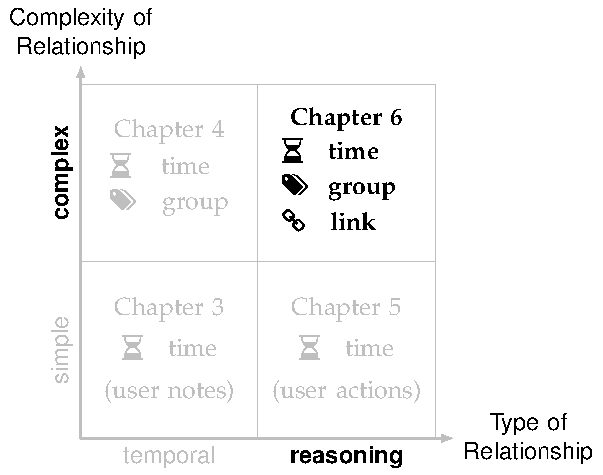
\includegraphics{work}
\end{figure}

\pagebreak

\section{Chapter Overview}
\lettrine{T}{he} previous chapter introduced a timeline visualization of automatically captured actions to enable researchers to explore reasoning relationships in the sensemaking processes performed by other people. In this last block of the thesis, we investigate whether and how analytic provenance can help people in their own \emph{ongoing} sensemaking processes. People often get lost while making sense of complicated tasks using big datasets over a long period. They may forget what they have done, may be unaware of where they are in the context of the overall task, and may be unsure where to continue. Visualizing the provenance of user actions to provide an overview of the sensemaking process could help address this issue. Also, during sensemaking, by allowing users to interact with their provenance information, they can externalize additional knowledge to the automatic capture such as through grouping and linking related information. This richly semantic organization could help users express and understand the relationship of their individual findings better and remember them more easily.

In this chapter, we introduce a visualization tool -- \emph{SenseMap} -- that enable users to explore \emph{complex reasoning relationships} of sensemaking through the visualization of provenance data with additional grouping and linking attributes, focusing on the context of \emph{browser-based online sensemaking}. We conducted a semi-structured interview with nine participants to explore their behaviors in online sensemaking with existing browser functionality. A simplified sensemaking model based on Pirolli and Card's model is derived to better represent the behaviors we found: users iteratively \emph{collect} information sources relevant to the task, \emph{curate} them in a way that makes sense, and finally \emph{communicate} their findings to others. A series of design workshops was followed to derive requirements, discuss designs, implement and test the prototype in an agile setting. SenseMap provides multi-linked visualizations of analytic provenance and enable users to curate and communicate their findings. To explore how SenseMap is used, we conducted a user study in a naturalistic work setting with five participants completing the same sensemaking task related to their daily work activities. All participants found the visual representation and interaction of the tool intuitive to use. Three of them positively engaged with the tool and produced successful outcomes. It helped them organize information sources, quickly find and navigate to the sources they wanted, and effectively communicate their findings.

A demonstration of SenseMap can be found at \url{https://vimeo.com/161322047}. The work of this chapter was published as:

\textbf{P. H. Nguyen}, K. Xu, A. Bardill, S. Betul, K. Herd, and B. L. W. Wong. SenseMap: Supporting Browser-based Online Sensemaking through Analytic Provenance. In \textit{IEEE Conference on Visual Analytics Science and Technology}, pages 91--100, oct 2016.

\section{Introduction}
People often get lost while solving complicated tasks using big datasets over long periods of exploration and analysis. They may forget what they have done, fail to find the information they have discovered before, and do not know where to continue. One approach is to capture and visualize user interactions in such a way that provides an overview of the sensemaking process to the user. In the World Wide Web context, the aforementioned problem is known as the \textit{disorientation} problem~\cite{Conklin1987}. One approach to address this problem is through a graphical browser history~\cite{Ayers1995,Hightower1998,Milic-Frayling2003}. It visualizes visited web pages and the linking relationships between them to help users to quickly see where they are in the network and to navigate to the page they want. However, when solving a sensemaking task online, which requires gathering, restructuring and reorganizing lots of information to gain insight, the disorientation problem becomes more severe and difficult to address. They do not just get lost in the hypertext space but also get lost in the task space. They may be unable to answer the following questions. What has been done so far? Where am I in the context of the overall task? What information should I search for next?

% Generally, what we did
In this chapter, we introduce a tool, \emph{SenseMap}, to support \textit{browser-based online sensemaking} through analytic provenance. We targeted this domain because many everyday sensemaking tasks such as travel planning are now performed online~\cite{Russell2008}.
We followed a user-centered, iterative design process to address the problem. First, user behaviors in online sensemaking are elicited through interviews. Then, a simplified sensemaking model based on Pirolli and Card's model~\cite{Pirolli2005} is derived to better represent these behaviors: users iteratively \textit{collect} information sources relevant to the task, \textit{curate} them in a way that makes sense, and finally \textit{communicate} their findings to others. A series of design workshops was followed to derive requirements, discuss designs, implement and test the prototype in an agile setting. SenseMap consists of three components: a \emph{browser view} that is a standard web browser with additional sensemaking support, a \emph{history map} that provides an overview of the sensemaking process, and a \emph{knowledge map} that allows users to curate the collected information. Communication support is provided in all three components.

To explore how SenseMap is used, we conducted a user study in a naturalistic work setting with five participants completing the same sensemaking task related to their daily work activities. Both quantitative data about user activities with SenseMap and qualitative data through semi-structured interviews were collected. All participants found the visual representation and interaction of the tool intuitive to use. Three of them positively engaged with the tool and produced successful outcomes.

SenseMap is freely available as a Chrome extension~\footnote{\url{https://chrome.google.com/webstore/detail/sensemap/agljnpanahlilmpipaeflmnjkiiecfjb/}}. In summary, it contributes
\begin{itemize}
\item A user study exploring user behaviors in online sensemaking with existing browser functionality, and a series of workshops followed up to generate requirements and discuss designs.
\item A visual sensemaking tool SenseMap supporting browser-based online sensemaking addressing all the derived requirements.
\item A user evaluation exploring how SenseMap is used in a naturalistic work setting and a discussion of insights gained and design lessons learned.
\end{itemize}
\section{Approach}
We followed a user-centered, iterative design process to develop SenseMap as a tool supporting browser-based online sensemaking. First, we identified current user behaviors in sensemaking using existing browser functionality. These behaviors led to the selection and subsequent development of a sensemaking model for user behaviors on the web. We conducted a series of design workshops to derive requirements from these user behaviors and model, then to design, build and test prototypes in an agile setting. Finally, the prototype was evaluated in a naturalistic work setting. \autoref{fig:sm-design-process} summarizes this process.

\begin{figure}[!htb]
	\centering
	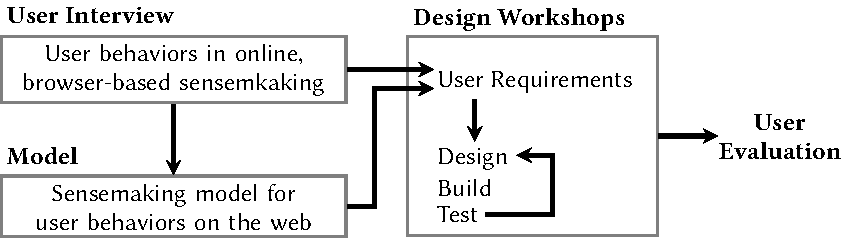
\includegraphics[width=\linewidth]{design-process}
	\caption{Summary of the design process.}
	\label{fig:sm-design-process}
\end{figure}

\subsection{Design Research}
We conducted a semi-structured interview with nine participants to explore their behaviors in  conducting online sensemaking for their daily work activities. The interview happened during a normal working day to access the currently open, in-use browsers of participants, as a representative artifact of their practice. Therefore, the participant's browser became the scaffold for the conversation and provided the ongoing probes as the conversation unfolded. This method also ensured that participants described about what they actually did rather than talking about what they thought they did or should do.

We took video of each interview with the camera showing the interviewee's laptop screen and their hand gestures. We also made screen recordings of each laptop while the interview was taking place. \autoref{fig:sm-design-research} shows the combination of hand gesture and laptop screen of a participant. Each interview began with the participant showing their currently open browser windows. Browser choice was discussed and then the ongoing conversations were guided by five browser functions: searching, tabs, windows, bookmarks and history, with participants illustrating their behaviors using their in-use browsers. These behaviors are summarized as follows.

\begin{figure}
	\centering
	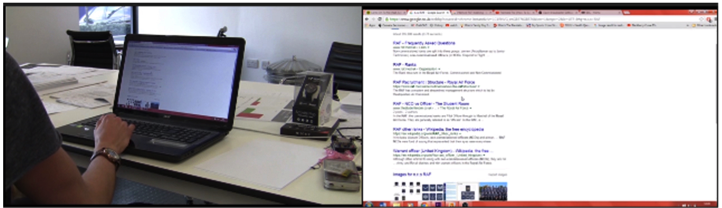
\includegraphics[width=\linewidth]{design-research}
	\caption{Interviewee's hand gesture and laptop screen.}
	\label{fig:sm-design-research}
\end{figure}

\paragraph{Starting Searches}
Opening a new tab preceded most searches. Users spoke about new tabs helping them to manage information, keep things separate and how they could go back to other pages that were relevant to their work activities and ongoing investigations.

\paragraph{Tabs}
Eight of the nine participants had a number of tabs open and categorized them as either: collections of tabs relating to current investigations or single points of access to commonly accessed services, e.g. social feeds, email etc. In further probing about the tab collections a number of shared behaviors emerged.

\begin{enumerate}
	\item Opening a new tab if ``significant'' information is found enabling the page to stay live in the browser.
	\item Opening Google search result links in a series of new tabs from one search page. Subsequent tabs were reviewed and then kept or closed based on their significance.
	\item Reordering tabs to develop a narrative. In all cases the narrative was described as flowing from left to right. The narrative was used by the participants to make sense of the information found, to develop more refined search strategies and terms where information was lacking, and to communicate their findings to others.
	\item All participants expressed anxiety about losing tabs when they were inadvertently closed or lost due to a system error and they all described the same recovery procedure using the recently closed tabs section of the History menu.
	\item The number of tabs in browser windows varied greatly across the participants. One participant diligently closed all tabs at the end of each ``work episode'' although sometimes they kept them open in a non-active window when at home and used a new window for private web browsing. Most described groups of seven to eight tabs that were currently in use for active projects. One user had over fifty tabs open in their main browser and twenty in their second browser, but they gave the same explanation for their presence, use and organization.
\end{enumerate}

\paragraph{Windows}
Only one user described the use of more than one window in the web browser. Similarly to Behavior 5, this enabled him to keep work-related tabs separate from private browsing.

\paragraph{Bookmarks}
There was considerable variance in the use of browser bookmarks although most had moved away from using them and relied instead upon tabs to keep relevant information live and accessible. Two participants had no bookmarks at all.  One participant saved some bookmarks, but these were not organized into groups, categories or folders. One participant described a behavior where they bookmark the contents of tabs at the conclusion of a project and organize these into named folders. However, they rarely revisited these bookmarks to use them to access information again, instead preferring ``Pinterest'' or relying on Google to find it again from a search term.

\paragraph{History}
None of the participants made use of the history menu to revisit pages or to make sense of recorded information. However, all of them used it to reestablish a tab if it had been inadvertently closed.

\subsection{Sensemaking Model}
We considered the relevance of extant sensemaking models to the elicited behaviors, principally Pirolli and Card's model and Data--frame model (Literature Review chapter, \autoref{sub:lr-sensemaking}). The iterative process of sensemaking described by Pirolli and Card effectively encapsulates the observed tab behaviors:

\begin{itemize}
	\item The \emph{foraging loop}: behaviors 1 and 2
	\item The \emph{sensemaking loop}: behavior 3
	\item Behaviors 4 and 5 indicate possible tool features rather than a step described in Pirolli-Card model.
\end{itemize}

The synthesis of our observed behaviors with the Pirolli and Card's model indicates a browser-based sensemaking process, during which information sources are held in a \textit{collection} of browser tabs (foraging loop), with each tab containing the provenance for the source. An ongoing \textit{curation} process (sensemaking loop) takes place where tabs are ordered into categories and a narrative sequence unfolds within such categorized groups. These groups and relationships represent the underlying schema. The results of the curation are then used to guide further more refined searches and, on completion, as a support to \textit{communicate} the findings to others. \autoref{fig:sm-refined-sensemaking-model} illustrates our refined model.

\begin{figure}
	\centering
	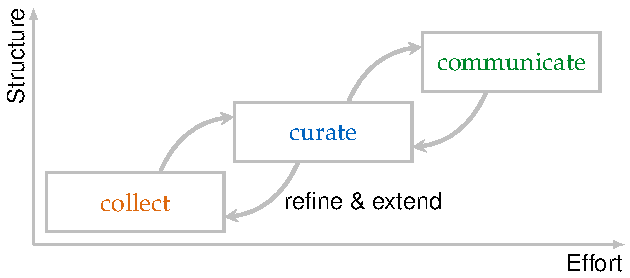
\includegraphics{refined-sensemaking-model}
	\caption{Our refined sensemaking model for user behaviors on the web.}
	\label{fig:sm-refined-sensemaking-model}
\end{figure}

\subsection{Design Workshops}
We organized a series of iterative design workshops to derive and satisfy requirements with an overall aim to support and augment current browser-based online sensemaking activities. In the first workshop, an initial design was proposed, detailing visual representation and user interaction. A prototype was built based upon this proposal, and subsequent workshops sought to develop this tool through the ongoing interplay between design, build and test in an agile setting.

We will describe the requirements next and present the interface design in \autoref{sec:sm-design}. Some of these requirements link directly to observed behaviors, some are inferred from our sensemaking model, and some are produced during creative design processes set within the constraints of the technology platform chosen.

\subsubsection{Collection Requirements}

\begin{enumerate}
	\item \textbf{Rich provenance}: enrich and make the provenance of information sources more visible to users. Currently, the provenance of tabs is only accessible when they are active and then only by a list of page titles (in Chrome, press and hold the browser's back button), which requires users to build their own schema that is external to the browser.
	\item \textbf{Easy revisitation}: provide quick and easy mean to revisit the information sources needed. Our interviews show that users often revisit their important tabs (Behaviors 1 and 2), but rarely use bookmarks and history. During a session, they rely on the tab titles, their memories or trial-and-error. However, tab titles are represented by a favorite icon and a truncated page title, which is a poor abstraction from the original source. This abstraction becomes poorer as more tabs are opened, making revisitation difficult when tab collections are large.
	\item \textbf{Location awareness}: provide an overview of the sensemaking process to address the disorientation problem~\cite{Conklin1987}, enabling users to know what they have done so far, where they are in the context of the overall tasks, and potentially guide the next step.
	\item \textbf{Preparation for curation}: provide highlight and annotation support for users, which can facilitate more elaborate thinking~\cite{Sedig2013}, and can serve as a step to assess the relevance of the information sources. The information representation should have different levels of richness depending on the assessed relevance.
	\item \textbf{Interruption \& Separation}: enable task switching without compromising the collection process; for instance, checking email or social feeds should not get recorded as part of the sensemaking process (Behavior 5).

	\setcounter{listnum}{\theenumi}
\end{enumerate}

\subsubsection{Curation Requirements}

\begin{enumerate}
	\setcounter{enumi}{\thelistnum}
	\item \textbf{Rich representation}: provide a rich abstraction of the information source allowing the user to quickly recognize it~\cite{Tauscher1997}. This also relates to the ``Easy revisitation'' and ``Location awareness'' requirements for Collection.
	\item \textbf{Spatial organization}: enable users to freely arrange information sources in both $x$ and $y$ dimensions to address the limit of a one-dimensional sequence of tabs being used to visualize multiple narrative threads (Behavior 3). Spatial organization plays an important role in sensemaking~\cite{Sedig2013}, especially with a large space~\cite{Andrews2010}.
	\item \textbf{Linking/unlinking}: enable further curation of these sources by establishing links, which is impossible with existing browsers. Linking and unlinking are also known to help users to produce more critical thinking~\cite{Sedig2013}.
	\item \textbf{Formal reasoning}: enable users to apply formal argumentation methods such as Toulmin's argument~\cite{Toulmin2003} or Wigmore's chart~\cite{Goodwin2000}. We think that they may be helpful when solving complex sensemaking tasks analytically.
	\item \textbf{Collection -- Curation}: enable users to see connections between the curated and collected sources, and to use these to inform further searches. This is to support the ``refine and extend'' direction in our sensemaking model (\autoref{fig:sm-refined-sensemaking-model}).

	\setcounter{listnum}{\theenumi}
\end{enumerate}

\subsubsection{Communication Requirements}

\begin{enumerate}
	\setcounter{enumi}{\thelistnum}
	\item \textbf{Complete picture}: provide a complete picture of the curated sources and the relationships that a user ascribes to them via their curation activity. Currently, it is impossible to see an overall picture of the curated sources and their categorization from the sequence of tabs.
	\item \textbf{Auditability}: enable users to refer to raw data as evidence supporting their reasoning, which is considered as an important characteristics in analytic presentation~\cite{Chinchor2009}.
	\item \textbf{Varied audience}: enable users to customize the curated set of information to suit various needs and backgrounds of the audience. This is also another important characteristic in analytic presentation~\cite{Chinchor2009}.
	\item \textbf{Sharing}: enable users to share both raw and curated sets of information with others. This is a first step toward a collaborative environment for online sensemaking.
\end{enumerate}
\section{Interface Design}
\label{sec:sm-design}

\subsection{Approach}
In the initial design session of the workshops, we considered all elicited requirements and agreed that SenseMap needs to:
\begin{enumerate}
	\item Capture web pages that the user visited, the sensemaking actions that happened there, and how the user arrived at those pages.
	\item Visualize the captured information in such a way that the user can understand what they have done, how things are connected, and what else they may do next.
	\item Support the user to curate the collected information according to its relevance, facilitate their reasoning, and communicate the findings. Also, this should not interfere with the original relationship among collected information so that the user can always use it as a reference.
\end{enumerate}

\subsection{Overview}
SenseMap consists of three views:

\begin{itemize}
	\item A \textit{Browser View} (\autoref{fig:sm-overview}A) that is a standard web browser with additional sensemaking support and provenance capture of actions happening there.
	\item A \emph{History Map} (\autoref{fig:sm-overview}B) that shows captured sensemaking actions with their page linking provenance while preserving their temporal order as much as possible to provide an overview of the sensemaking process (Point 2 above).
	\item A \emph{Knowledge Map} (\autoref{fig:sm-overview}C) that allows users to curate the collected information. This map is separate from History Map to preserve the semantic and temporal structure of the captured information (Point 3 above).
\end{itemize}

\begin{figure}
 	\centering
 	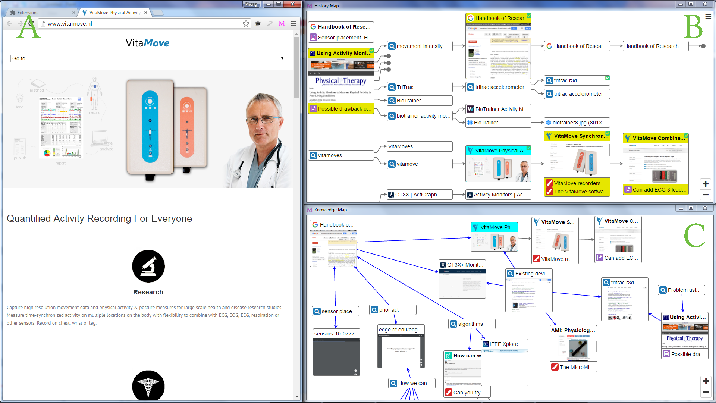
\includegraphics[width=\linewidth]{overview}
 	\caption[Three linked views of SenseMap]{Three linked views of SenseMap. \textbf{A:} This is the standard browser with additional sensemaking and provenance support. \textbf{B:} The history map captures and visualizes user actions to provide an overview of the sensemaking process. \textbf{C:} The knowledge map enables users to curate and make sense of the most relevant information to their tasks.}
 	\label{fig:sm-overview}
\end{figure}

In the next three sections, we will discuss these views and how they address the design requirements. \autoref{fig:view-and-process} summarizes the support that each view provides.

\begin{figure}
	\centering
	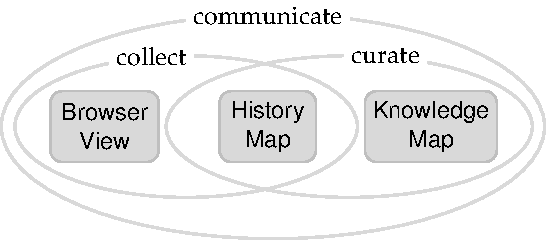
\includegraphics{view-and-process}
	\caption[Views and the sensemaking subprocesses they support]{Views and the sensemaking subprocesses they support. \emph{Collection} is supported in Browser View and History Map. \emph{Curation} is supported in History Map and Knowledge Map. \emph{Communication} is supported in all three views.}
	\label{fig:view-and-process}
\end{figure}

\subsection{Browser View}
This is a standard web browser with provenance capture and additional sensemaking support. The content and method to capture such provenance is the same as in the previous chapter, \autoref{sub:sp-provenance}. Additional features augmented to the browser are described as follows.

Highlighting and annotation are essential editing support. They allow users to mark relevant information and to assign their own interpretation (Requirement 4). A new option ``Highlight'' is added to the context menu when a passage of text is selected allowing the user to highlight it. That text becomes clickable allowing the user to either write a note or remove the highlight.

When a web page is visited, SenseMap takes a screenshot and uses it to represent the page in the history map (\autoref{sub:collection}). It is intended to help the user to quickly recognize web pages that have been visited (Requirement 2). However, that screenshot may not reflect perfectly the main content of the web page, especially when the picture contains lots of text. To address this issue, we allow the user to assign a custom representative image to a web page. This can be done by simply right-clicking on any images in the web page and select ``Set as Page Image'' option in the context menu.

\subsection{History Map}
\label{sub:collection}
This map provides an overview of the sensemaking process using the captured actions and their provenance (\autoref{fig:sm-overview}B).

\subsubsection{Visual Representation}
An action is represented as a bar with an icon indicating its type and text showing the contextual information. Icons help users recognize action types faster and we use the same icon set as shown in the previous chapter, \autoref{fig:icon-list}. If the action type is the default \textit{browsing}, the favorite icon of its web page is used instead. The contextual text is important to understand what the action is about and it is truncated up to a certain length to fit to the limited space. \autoref{fig:action-bar} shows an example of a keyword search action.

\begin{figure}
	\centering
	
\includegraphics[width=.3\linewidth]{action-bar}
	\caption{Action bar for a keyword search ``visual analytics conference''.}
	\label{fig:action-bar}
\end{figure}

Highlights and annotations of the same web page are grouped together as in \autoref{fig:action-highlights}. They are located in separate rows below the web page title. By default, just a few highlights and annotations are shown to ensure a reasonable height for the page. All of them can be revealed using a menu available when hovering on any highlight or annotation.

\begin{figure}
	\centering
	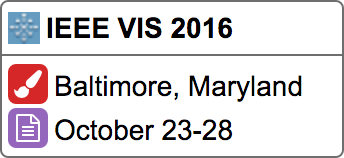
\includegraphics[width=.3\linewidth]{action-highlights}
	\caption{A page with one highlight and one note.}
	\label{fig:action-highlights}
\end{figure}

To provide a connection between the history map and the browser view, the action bar corresponding to the active browser tab is highlighted in cyan. Pages that have been opened but have not seen yet (could be the result of opening links in new tabs) are shown with a dashed border, which may help to remind the user to read them. \autoref{fig:action-active-not-seen} shows an example of pages with these two states.

\begin{figure}
	\centering
	
\includegraphics[width=.6\linewidth]{action-active-not-seen}
	\caption[Representation of active page]{The user is active on a search result page (left bar) and opens a link in a new tab (right bar).}
	\label{fig:action-active-not-seen}
\end{figure}

\subsubsection{Layout}
\label{sub:sm-layout}
Seeing the provenance of a web page is important to the user (Requirement 1). Currently, it can only be seen if the user presses and holds the browser's back button. This provenance information is not even available if a page is open in a new tab. In the history map, linking relationships between two pages are always visible and illustrated by an arrow pointing from the source to the target (\autoref{fig:action-active-not-seen}). For example, if the user clicks on a link in page $A$ yielding to page $B$, an arrow from $A$ to $B$ will be added to show this relationship. Showing links between pages can reveal branching structures such as when multiple pages are opened in new tabs from the search result page. This provides richer provenance information and easier access for the user compared to a linear list of visited pages as in current browsers.

Technically, all pages and links in the history map form a \textit{forest}, where tree roots are pages that do not have a parent page such as pages opened by entering the URLs manually. Temporal information of sibling pages are indicated by the order of them: earlier opened pages are placed above later ones. This also helps maintain the mental model for the user about their process: the order of pages are never changed; and a new page is added either on the right side of the page triggering its opening or at the bottom of the map when such linking does not exist. A virtual node is then added and connected to all tree roots to form a single tree. We use the compacted tree layout in \textit{jgraph} library~\footnote{\url{https://www.jgraph.com/}} to produce the location of pages (\autoref{fig:sm-overview}B).

Temporal information shows the order of actions that the user has taken, and the branching and linking relationships reveal their semantics. At a lower level, highlighting the active tab in the layout as described earlier helps the user know where the page they focusing (active) page in the context of the overall process. Both of these supports address Requirement 3.

\subsubsection{Preparation for Curation}
The history map displays all captured actions; however, probably not all of them are equally important and relevant to the sensemaking task. Therefore, it is necessary to allow users to assess the relevance of the collected information. We use the term \textit{node} to refer to either a simple search action bar or a page containing many highlights -- a node in the tree layout. Three levels of relevance are provided, all through the menu available when hovering a node.

\begin{enumerate}
	\item If a node is completely irrelevant, the user can \textit{remove} it.
	\item If a node is not quite relevant but the user wants to keep it to have a look at some point, they can \textit{minimize} it.
	\item If a node is very relevant, the user can \textit{favorite} it.
\end{enumerate}

When a node is removed, it and its links are removed from the map. When a node is minimized, it is collapsed into a small circle. This enables users to focus on other nodes and also save the display space. Favorite nodes are displayed with a yellow background and a thumbnail of the captured screenshot to increase their recognizability. \autoref{fig:action-minimize-favorite} shows an example of minimized and favorite nodes.

\begin{figure}
	\centering
	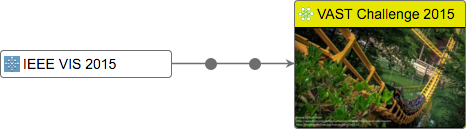
\includegraphics[width=.75\linewidth]{action-minimize-favorite}
	\caption[Pre-curated nodes]{Nodes are pre-curated: two irrelevant nodes in the middle are minimized, whereas the last one is set favorite.}
	\label{fig:action-minimize-favorite}
\end{figure}

\subsubsection{Scalability}
\label{sub:sm-scalability}
Nodes can reduce their size through zooming to accommodate more nodes within the visible part of the history map. By default, all nodes have the same width and the same maximum height, which allows a few words of the contextual text visible, and a reasonably large thumbnail image, which may help users recognize the visited pages. For each smaller level, both the node width and the number of highlights are reduced. The node height is adjusted so that the ratio between it and the node width remains unchanged. At the smallest level, only the action type icon or a small thumbnail image is shown. \autoref{fig:zoom} shows an example of different zoom levels applied onto the same node.

\begin{figure}
	\centering
	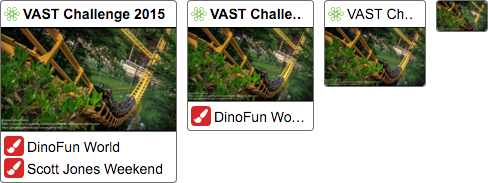
\includegraphics[width=.85\linewidth]{zoom}
	\caption{The same node with four zoom levels.}
	\label{fig:zoom}
\end{figure}

Node zoom level is explicitly controlled by the user using simple plus/minus buttons. When the collection of nodes exceeds the visible area, the user can pan the map to see them.

\subsubsection{Revisitation and Interruption}
When an action is captured, its web page's URL is also recorded. Clicking on a node opens its associated web page. This releases the user from worrying about losing browser tabs. Moreover, the additional branching and linking structure of the layout could help the user find information faster than the linear list of page titles in the History feature of the standard web browsers (Requirement 2).

To provide a more fine-grained bookmarking and navigation than the web page URL level, revisiting a captured highlight brings the user to the exact text being highlighted. This is made possible by capturing the relative location of the highlight with respect to the root of the web page.

In the real world environment, the user may have many sensemaking tasks happening at the same time (Requirement 5). Even while working in a single task, the user may do some other things irrelevant to the task such as checking email and social feeds. Therefore, always capturing user actions and putting them into a single place will result a huge mix of unrelated information. To address this issue, we allow the user to create separate collections of information for different tasks. The user can also pause the information capture and resume when needed.

\subsection{Knowledge Map}
This map allows users to curate the information displayed in the history map (\autoref{fig:sm-overview}C).

\subsubsection{Visual Representation}
The curation process starts by adding nodes from the history map to the knowledge map. This is done via the \textit{Curate} button in the menu available when hovering over a node. Nodes in the knowledge map have the same visual representation with those in the history map. The only difference is that thumbnail images of curated nodes are always made visible to improve their recognizability (Requirement 6).

\subsubsection{Spatial Organization}
The limit of single dimensional ordering tabs from left to right is addressed in the knowledge map through the spatial organization of nodes (Requirement 7). The user can freely move nodes by simply dragging them around. This enables the user to spatially group nodes and to assign different meanings to them. \autoref{fig:free-movement} shows an example of a knowledge map with three clear groups based on their locations.

\begin{figure}
	\centering
	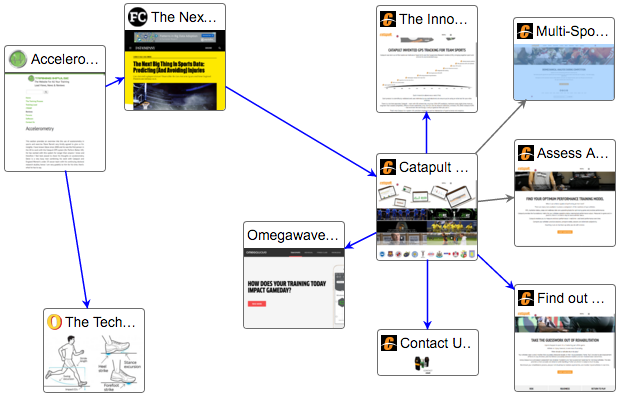
\includegraphics[width=\linewidth]{free-movement}
	\caption[An example of knowledge map]{A knowledge map with three clear groups of nodes as the result of free movement.}
	\label{fig:free-movement}
\end{figure}

\subsubsection{Linking/Unlinking}
Besides spatial grouping, seeing the casual relationships between collected information is also important to users in supporting sensemaking (Requirement 7). A conventional representation is used to show this relationship: an arrow pointing from the cause to the effect. The user can add a casual relationship by clicking on the ``cause node'', holding it for half a second until the cursor changes to an arrow, then  releasing the mouse on the ``effect node''.

When nodes are added to the history map, the provenance links among them are also copied to the knowledge map to provide an initial understanding of existing relations. Different colors are used to distinguish user-added links from provenance links.

\subsubsection{Formal Reasoning}
Currently, SenseMap does not support any formal argumentation methods. However, the flexibility of spatial organization and relationships establishment could help the user apply their reasoning strategies~\cite{Sedig2013}. For instance, users can draw a link from a ``hypothesis'' node to its evidence. Then, they can move all supporting evidence nodes to one area and all counter evidence nodes to a different location to distinguish the two groups.

\subsubsection{Collection -- Curation}
All nodes in the knowledge map appear in the history map, but the other direction is not always true because only relevant and important nodes may be curated. To help the user quickly recognize which nodes in the history map are already curated, a green ``tick'' icon is superimposed at the top right hand corner. Also, hovering a node in one map will highlight that node, if it exists, in the other map.

\subsubsection{Scalability}
By default, the knowledge map may only able to show several tens of nodes, which might be enough for a short sensemaking session. When the session is longer and the size of the map increases, semantic zooming (the same as in \autoref{sub:sm-scalability}) could help users manage the map in a certain extent. Addressing a larger map is our future work.

\subsection{Communication}
The final organization of curated information provides a complete picture of the sensemaking task, including the most important and relevant information to the users, which makes it ideal for them to present their findings (Requirement 11). If the process is of interest, the history map can be used alongside the knowledge map. Moreover, the user can refer to raw data, via node revisitation, to support their presentation (Requirement 12).

Both the history and knowledge maps can be saved as local files and loaded later. This allows users to share their maps (Requirement 14). Also, the user can create multiple copies of knowledge maps based on the same history map allowing customizing for various presentation purposes (Requirement 13).

\subsection{Implementation}
SenseMap is implemented as a Chrome extension based on the D3 visualization library~\cite{Bostock2011}. Chrome was chosen because of its high popularity. This decision was also confirmed in the initial interviews with seven out of nine participants using Chrome. Highlighting and annotation require modification of the web page structure, thus are implemented as content scripts using Chrome extension API. The provenance capture and action detection are implemented using the same method as in the previous chapter, \autoref{sub:sp-impl}.

%The three views communicate using \textit{messaging passing} mechanism provided by Chrome extension API. When an interaction occurs in one view, it sends a message to notify all other views. Each view constantly listens and responds to such messages.
\section{Evaluation}
We conducted a user-centered evaluation of SenseMap in a naturalistic work setting to explore its effectiveness in providing the desired support for sensemaking through the \emph{collect -- curate -- communicate} process. 

\subsection{Method}
%goal, overview setup
We recruited five participants who were all working as junior designers and engineers in an innovation center. The participants were all introduced to the tool, trained in its operation and given thirty minutes to try out the tool with support, before being given the task. Each participant installed the tool on their own device; all participants were using laptops (three Apple Macs and two Windows) -- and one participant had a second larger monitor connected. The participants conducted the task in their normal working environment (\autoref{fig:sm-evaluation-settings}) over a two-hour period.

\begin{figure}
	\centering
	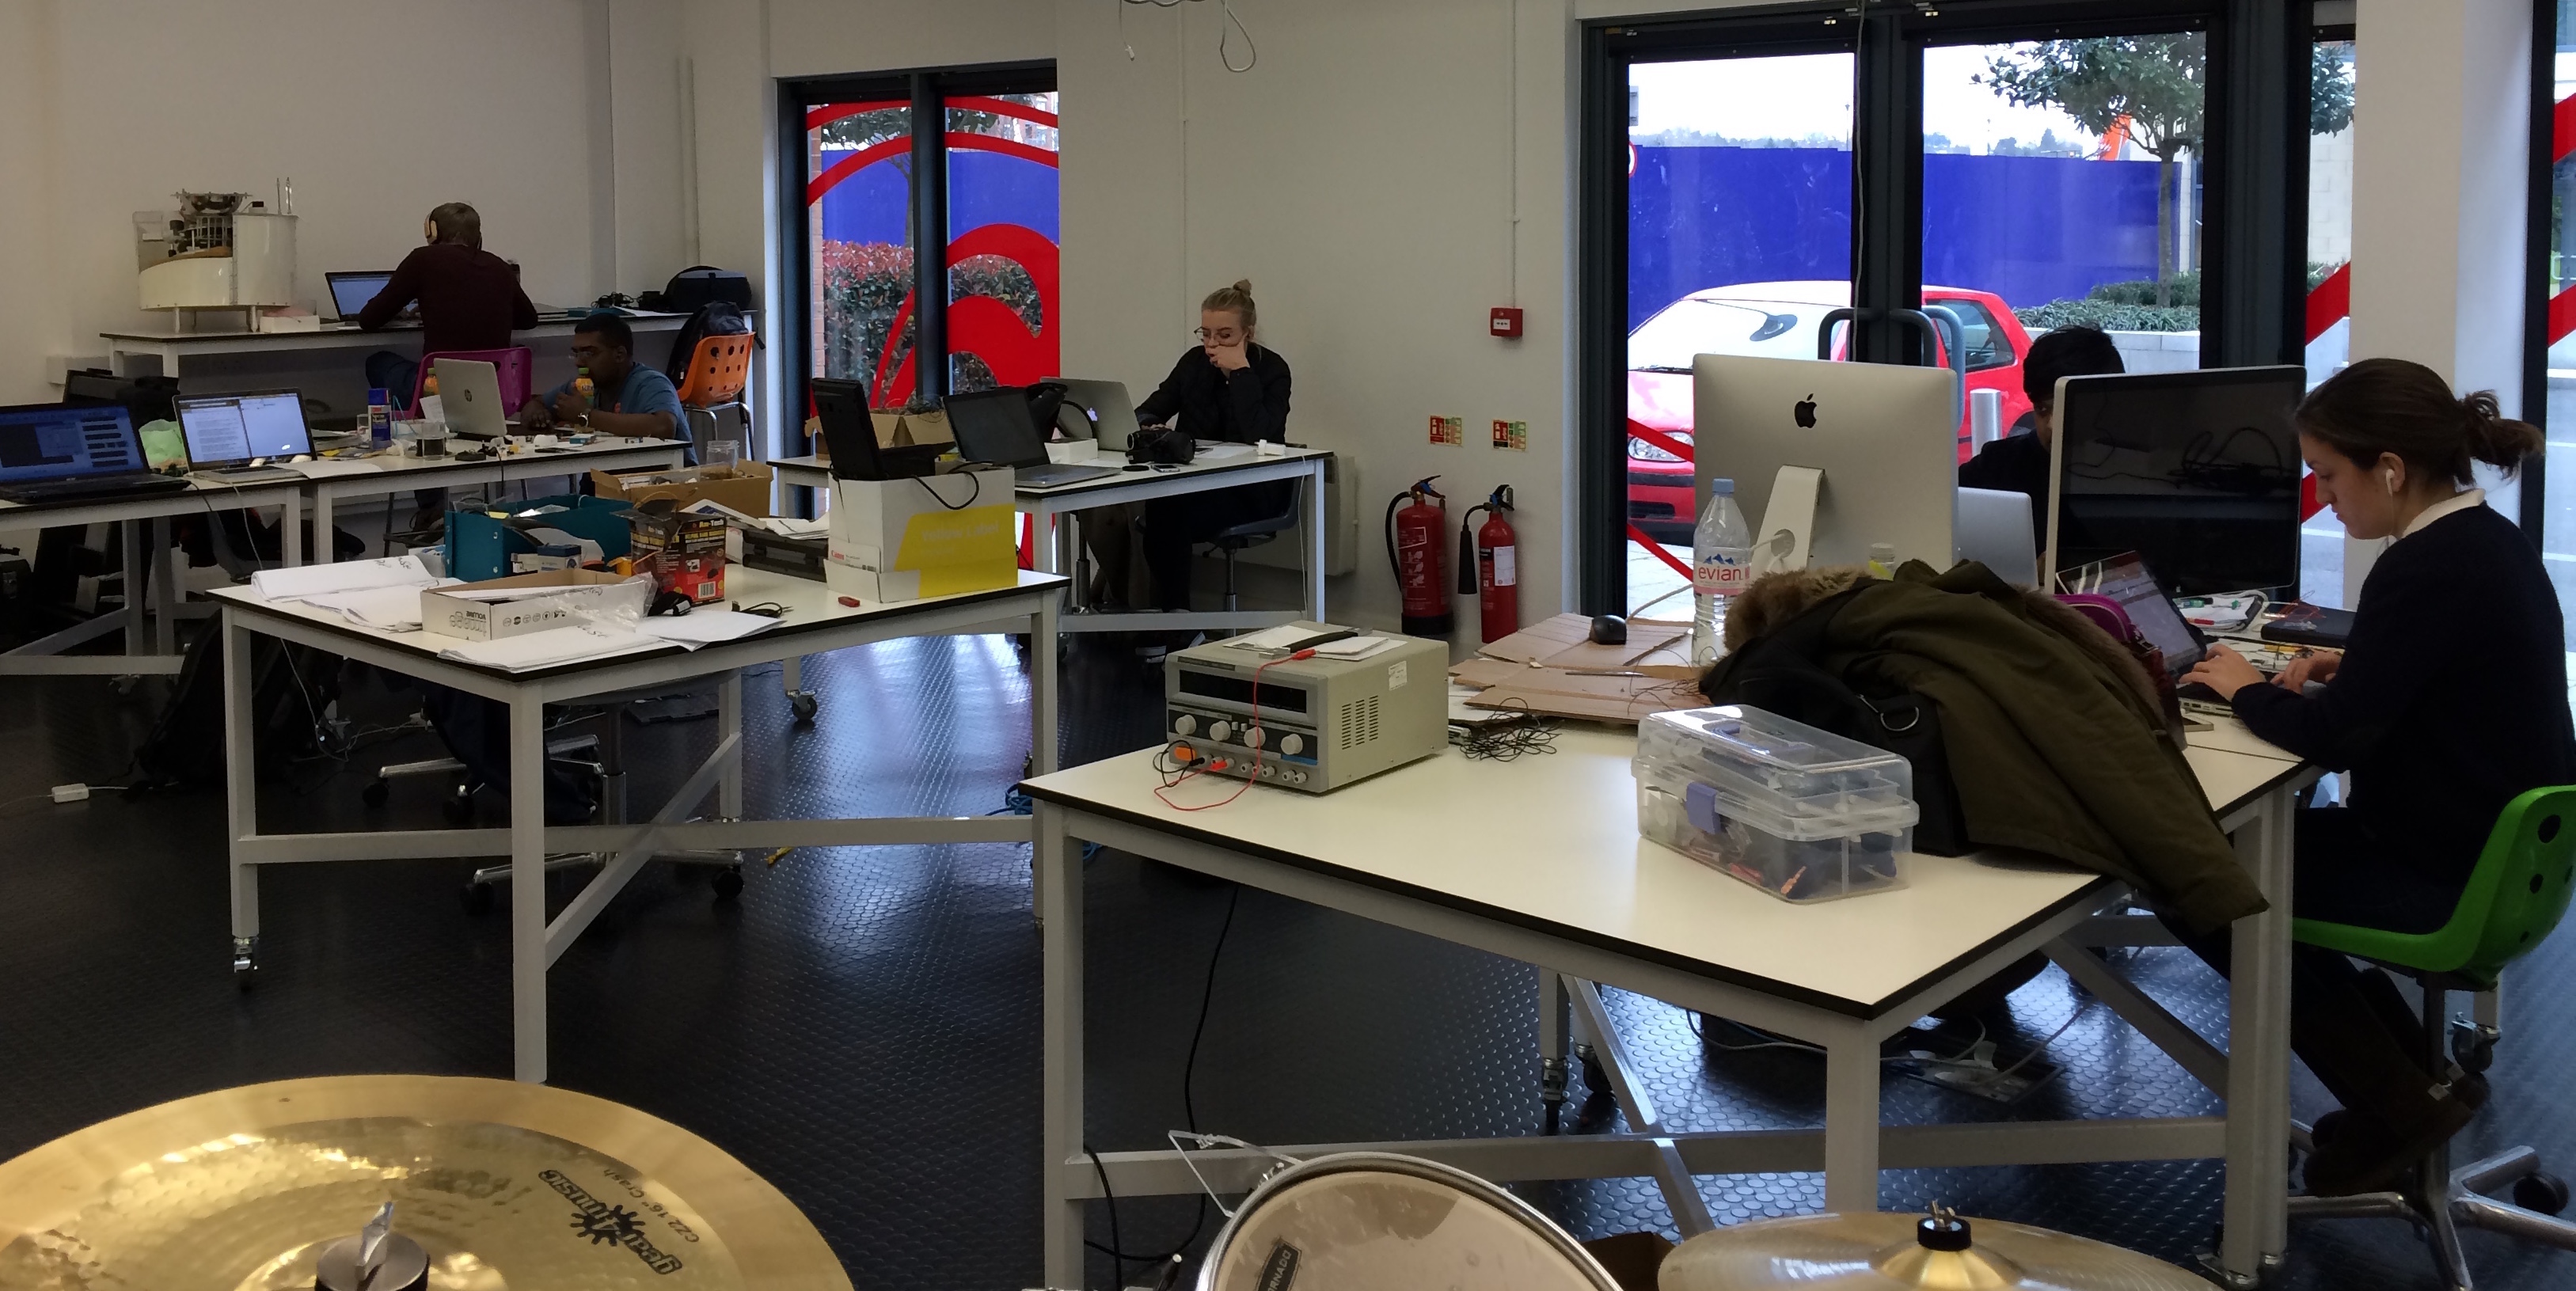
\includegraphics[width=\linewidth]{evaluation-settings.jpeg}
	\caption[Naturalistic work setting in the evaluation]{The working environment of the participants, which was also used in the evaluation to ensure a naturalistic work setting.}
	\label{fig:sm-evaluation-settings}
\end{figure}

%task
The task was devised to reflect normal work activities for these participants in the early research phases of an innovation project. We focused the task on technology selection and deployment, requiring them to collect and curate information on a variety of interrelated areas and then to communicate their findings. Participants were given the task in written form, and it was discussed to clarify any points of confusion or ambiguity. They were asked to complete the following task while using SenseMap to record and present their findings: ``We need to use accelerometers to measure movement intensity in ambulatory subjects and naturalistic settings, for up to 1 week. We need to find out about (in no order of priority): prior art, placement of devices, algorithms, commercial products and APIs, bespoke approaches, and anything else you feel relevant.''

At the end of the two-hour period we conducted an individual, semi-structured interview with each of the five participants. The participants were asked to present their findings, describe the process that they used to reach these findings using SenseMap, and to reflect upon their experience. We also collected interaction logs to explore how participants used SenseMap in their sensemaking activities over time including the timing (when), content (what) and position (where). All sensemaking features supported by SenseMap were captured such as highlighting and annotation in the browser, relevance assessment in the history map, and node movement in the knowledge map. Other standard interaction in the browser including window focus, lost and mouse, keyboard events were also captured.

\subsection{Data Analysis}

\subsubsection{Quantitative Features}
The quantitative data showed two distinct engagement profiles; i.e., how the participants engaged in the sensemaking process and interacted with SenseMap. \autoref{table:knowledge} shows the complexity of knowledge maps produced by all participants, indicating how much they were engaged with the tool. Also, \autoref{fig:evaluation-curation-histogram} shows the histogram of curation activities for all participants, allowing us to understand when the participants were most engaged with the tool and what they were doing.

\begin{table}[!htb]
	\centering
	\sffamily\small
	\caption{Knowledge Map produced by participants.}
	\label{table:knowledge}
	\begin{tabular}{ccc}
		\toprule
		\textbf{Participant} & \textbf{Number of nodes} & \textbf{Number of links} \\
		\midrule
		P1 & 10 & 12 \\
		P2 & 26 & 26 \\
		P3 & 6 & 7 \\
		P4 & 5 & 2 \\
		P5 & 35 & 35 \\
		\bottomrule
	\end{tabular}
\end{table}

\begin{figure}
	\centering
	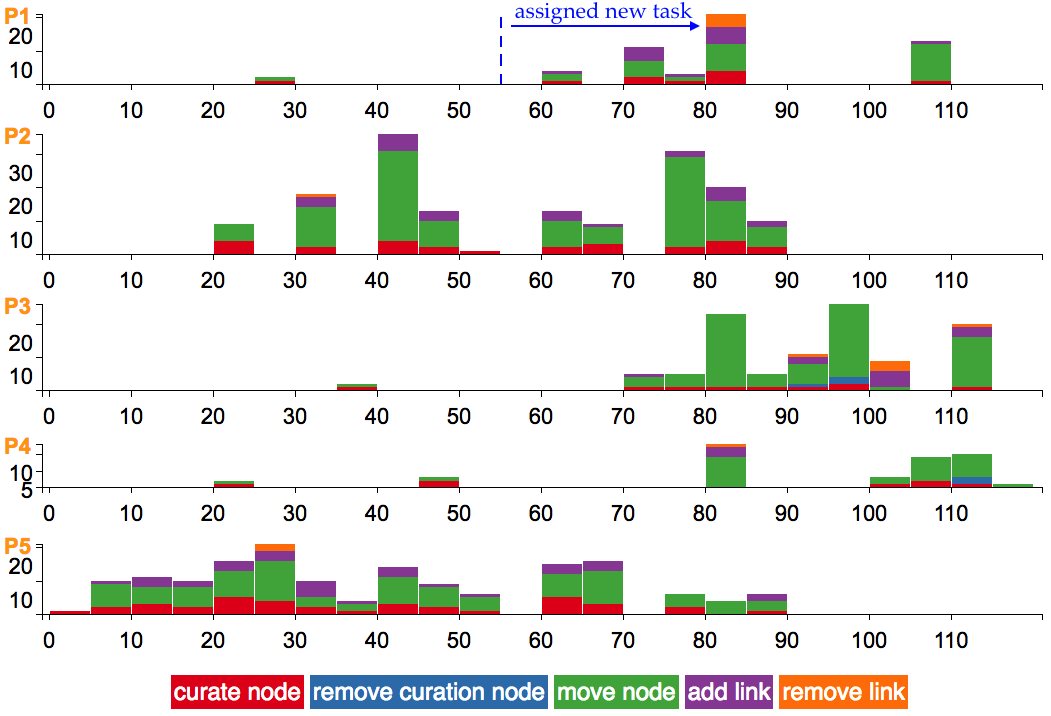
\includegraphics[width=\linewidth]{evaluation-curation-histogram}
	\caption[A histogram of curation activities for all participants]{A histogram of curation activities for all participants, with each bin spanning  5 minutes. Vertical axis shows the number of times the activities were performed.}
	\label{fig:evaluation-curation-histogram}
\end{figure}

\paragraph{High Engagement}
P5 was the first to curate and had the most detailed knowledge map with 35 nodes and 35 links. P2 had a similar profile with early and regular interaction with their window contents. P2 had the second most detailed knowledge map with 26 nodes and 26 links (\autoref{fig:sm-overview}C shows part of it). P1 began the trial with uncertainty due to a lack of technical knowledge of the task. The task was contextualized for P1 helping him to relate it more closely to his expertise. P1 began productive engagement with SenseMap at a later stage resulting in a similar engagement profile to P2 but compressed into a shorter timeframe (starting after around 55 minutes). P1 had the third most detailed knowledge map with 10 nodes and 12 links even though he only spent his second hour for the task. These participants share the same pattern --  \textit{curate early, curate often} -- and it relates to the interplay between collect and curate in our sensemaking model, through refining searches and extending the schema.

\paragraph{Low Engagement}
P3 did some minor curation activities early in the sensemaking process, but there was a considerable rise in the last third of the task time. There were only 6 nodes and 7 links in the final knowledge map with an indeterminate linking structure.

P4 did some minor curation activities with a short focus after an hour and more toward the end of the task. P4's interaction profile is notable for long and frequent periods of inactivity. P4 had only 5 nodes and 2 links in their final knowledge map with an indeterminate linking structure (\autoref{fig:Magda}).

\begin{figure}
	\centering
	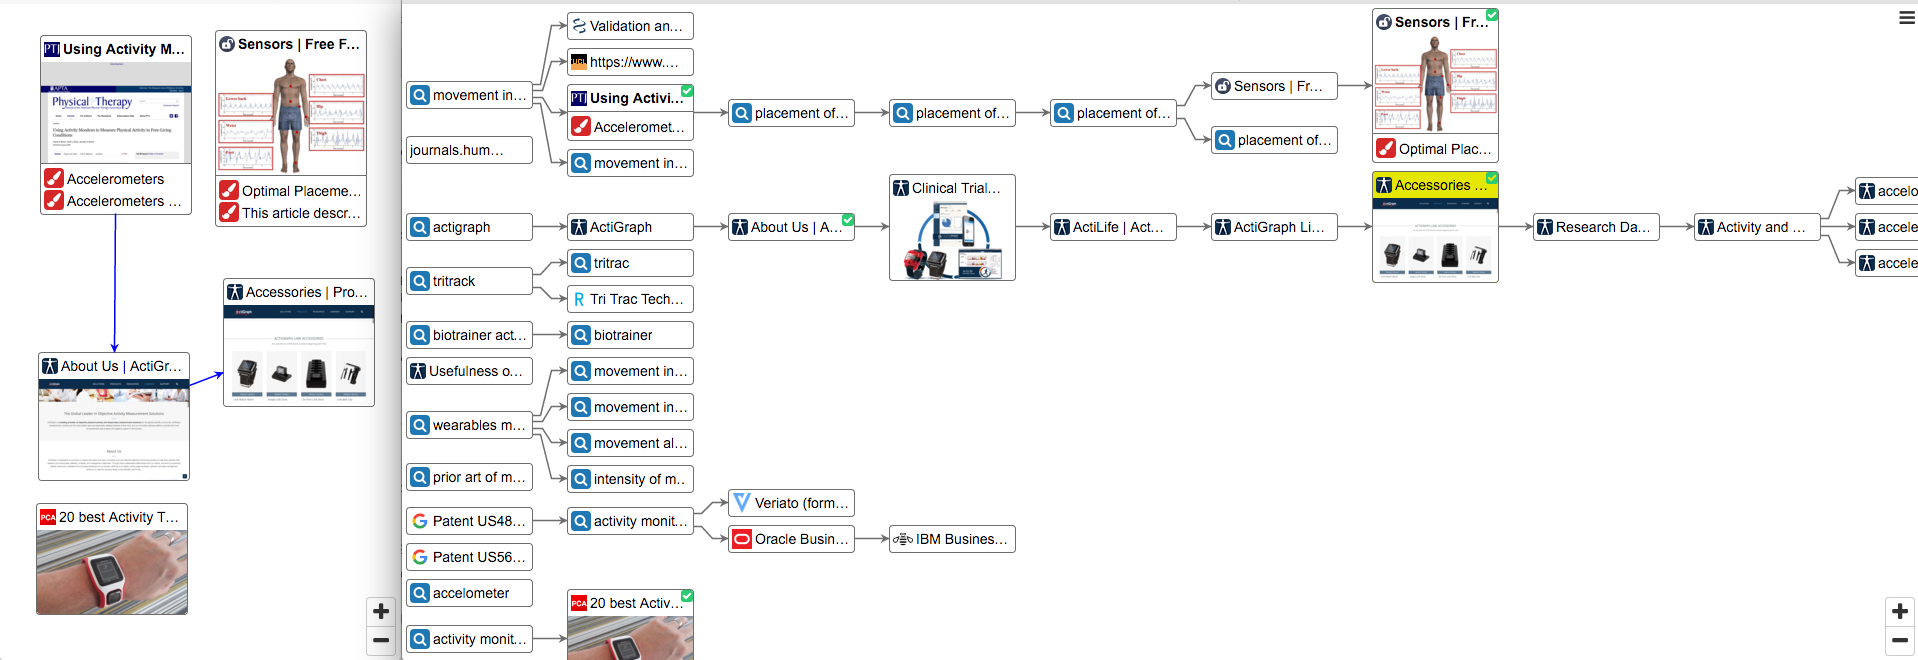
\includegraphics[width=\linewidth]{screenshots-evaluation/P4-Magda}
	\caption[Knowledge map and history map of P4]{P4: Knowledge Map (left) and History Map (right). P4 successfully moved a key document into the curation space, but subsequent schema is scant.}
	\label{fig:Magda}
\end{figure}

\subsubsection{Qualitative Features}

\paragraph{F1 -- Communication}
Did the participants use the knowledge map to communicate their findings? Had they successfully curated their schema through clusters, linked branches or other coherent structures? Had they constructed a narrative to explain their schemas?

\textbf{Positive: P1, P2, P5}. All had arranged their detailed knowledge maps as linked clusters from a key document. P1 and P2 were both able to provide a very coherent narrative about their findings. They confidently used the knowledge map to explain their findings, used links and clusters to explain relationships and recommendations, and clicked on nodes to access the original information sources in the browser view. P2 felt confident that he had completed the task in the time allowed and felt that the tool had helped him become more thorough, systematic and organized. P1 had low confidence in his technical expertise when he began the task, but after the task was recontextualized for him, he made considerable progress. He was pleased with the visual representation and interaction of the knowledge map, referring to it as a ``mind map'' -- a knowledge mapping process that he often uses. P5 was less able to provide narrative of his findings even though he had the most detailed knowledge map. He felt that he had not completed the task and was unsure about some of the technical aspects of it, which may have had some bearing on this. He was very positive about the use of the tool.

\textbf{Negative: P3, P4}. Neither of them were able to use their knowledge maps to communicate their findings, referring instead to their history maps. Both saw much potential in the tool to assist in sensemaking activities, but were less positive about their experience of it.

\paragraph{F2 -- Window Display}
Were participants able to work with their desired browser window size and effectively display or switch between windows during the task?

\textbf{Positive: P1, P2, P5}. P5 had a second monitor connected and was able to work with a full-screen browser window on his laptop as his point of focus. The two maps were arranged on the second monitor, each taking half of the screen, and the monitor was behind his laptop (\autoref{fig:evaluation-two-monitors}). He enjoyed this setting and referred to the external monitor as a second-brain. P1 and P2 both resized windows, but were adept at switching between them, and demonstrated fluidity in this during their interviews. P2 had arranged all three windows to be nearly full-screen and arranged them as an overlapping stack, so he could see the edges of all windows at all times. He also used the three-finger swipe on his Mac to minimize and show all windows and to switch between them.

\begin{figure}
	\centering
	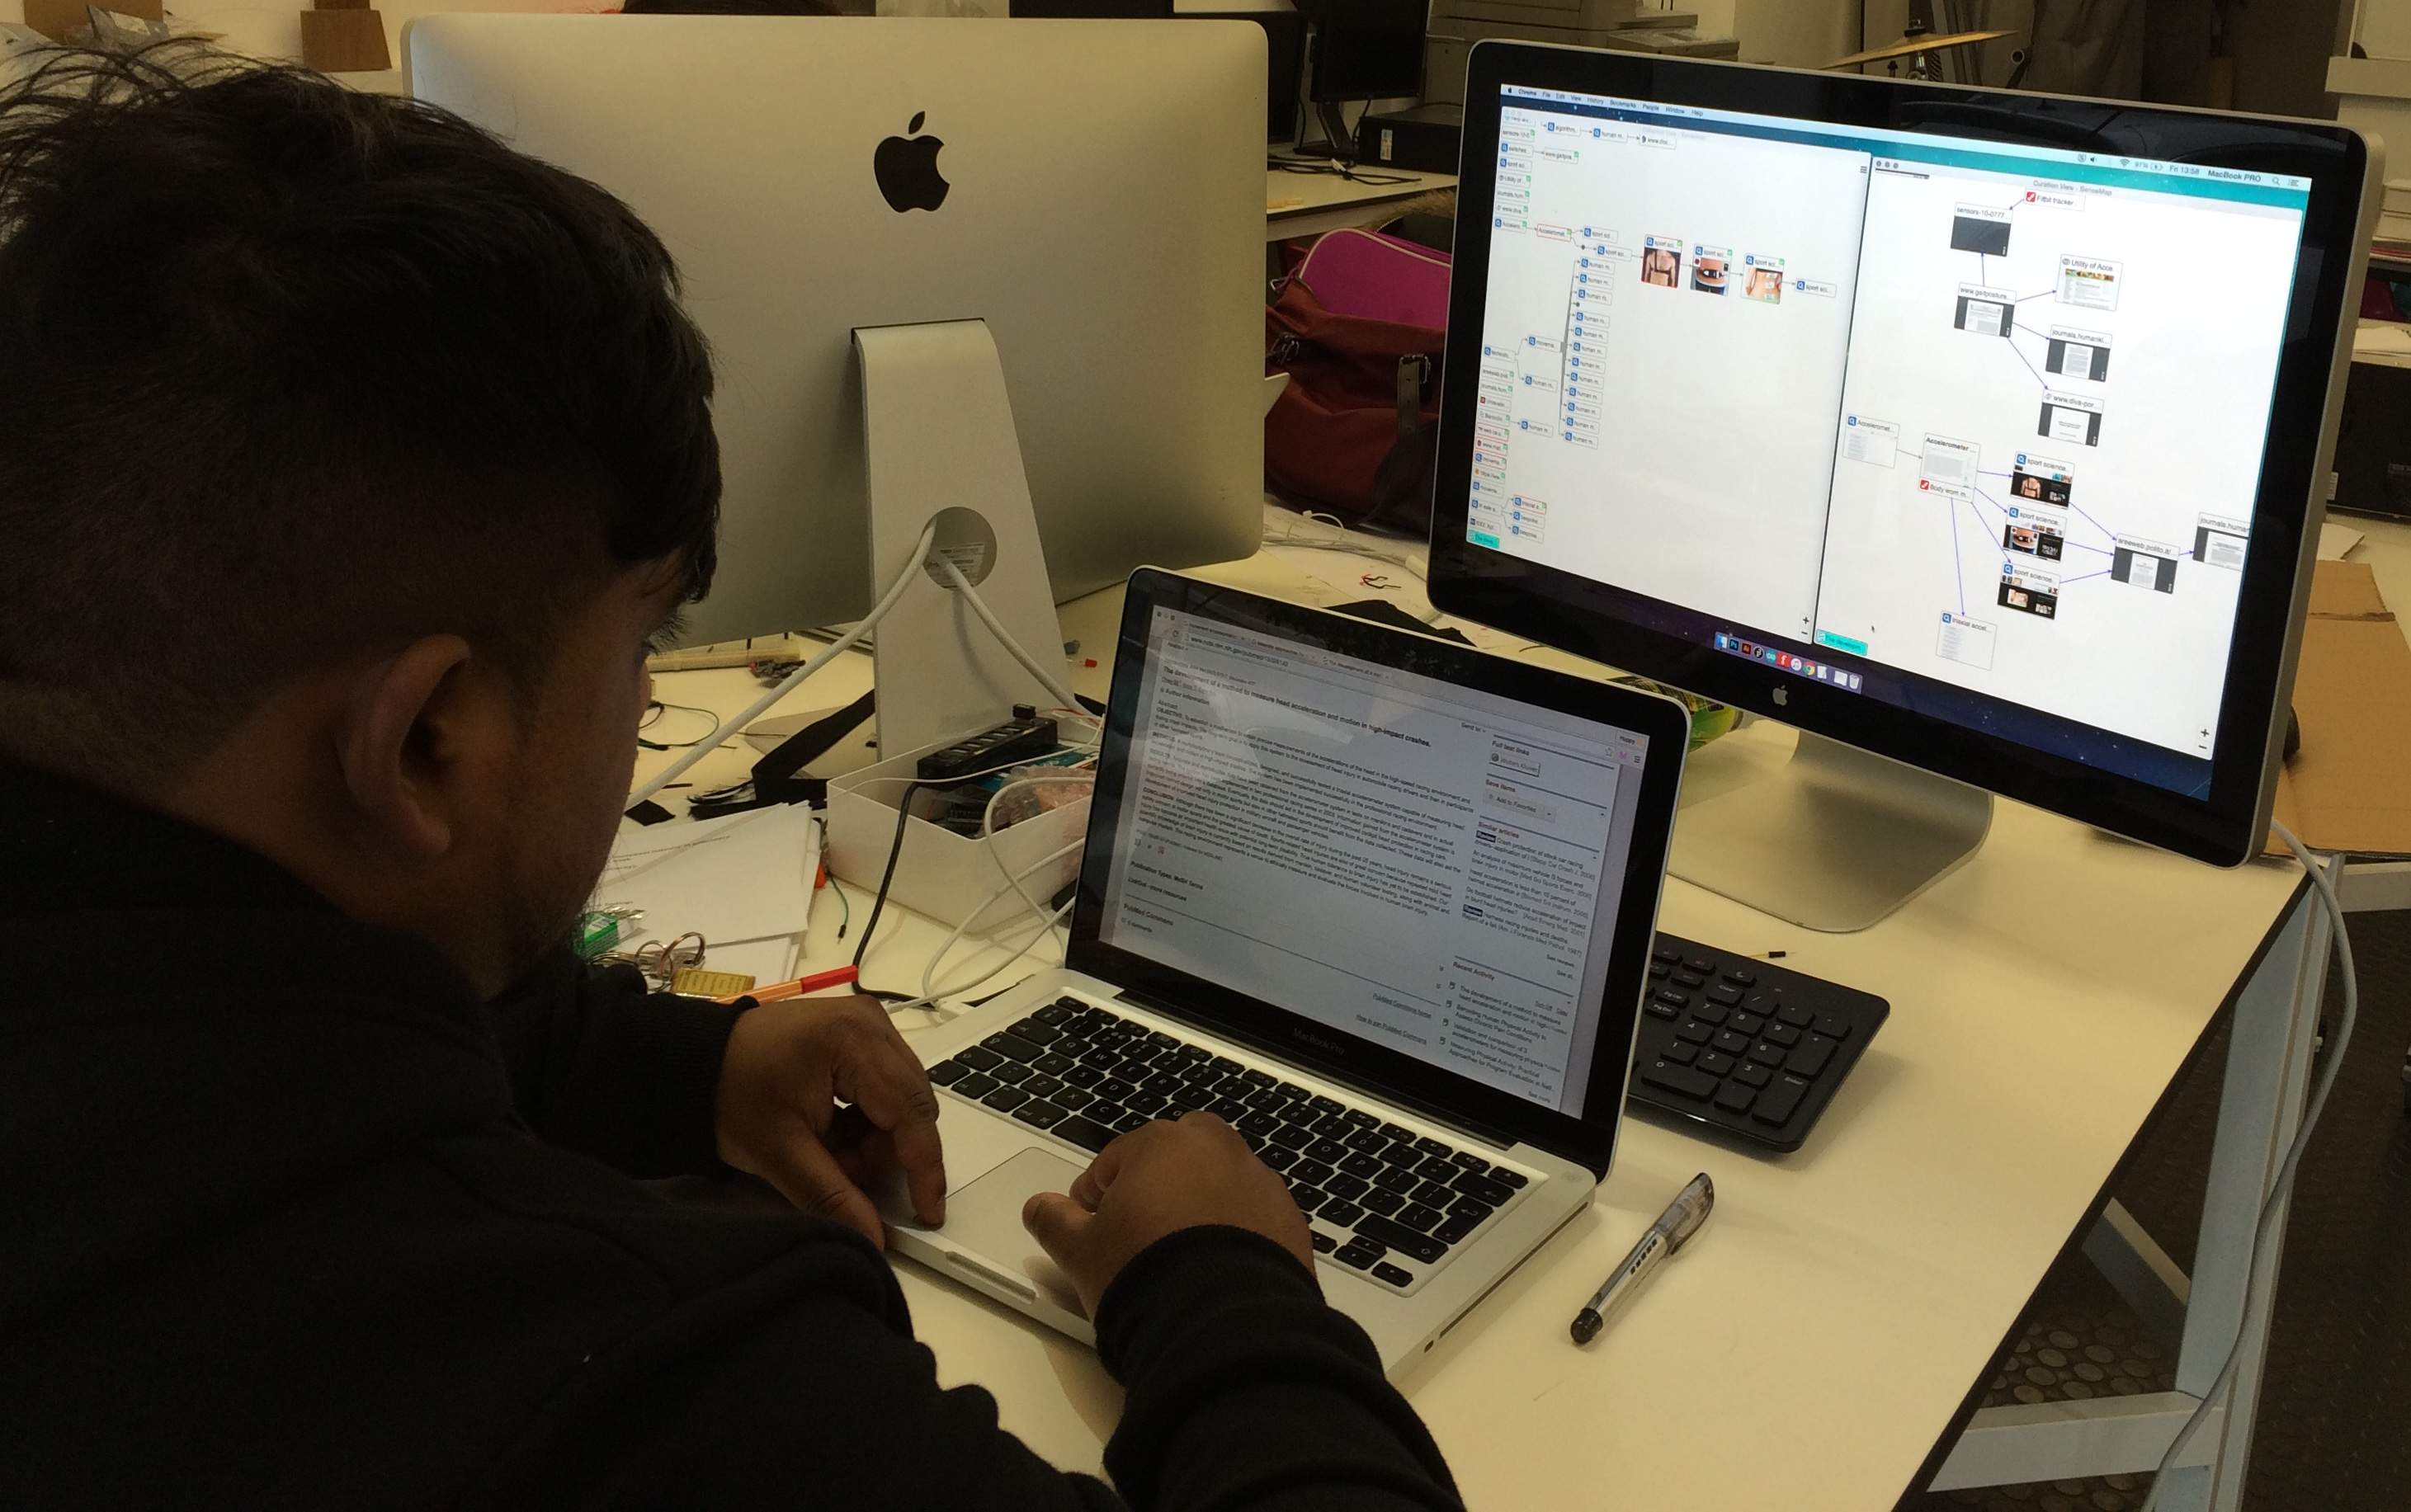
\includegraphics[width=\linewidth]{evaluation-two-monitors.jpeg}
	\caption[P5 with two monitors]{P5 with two monitors, comfortably interacting with all three views of SenseMap.}
	\label{fig:evaluation-two-monitors}
\end{figure}

\textbf{Negative: P3, P4}. Both of them reverted to full-screen browser windows and expressed a strong preference for this. P3 ignored the history map after losing reassurance that the tool could support him in his task. P4 reset the browser view to full screen, ignored the history map, and then lost track of the meaning of the collection when she returned to it.

\paragraph{F3 -- Keeping Track}
Did the participant understand and keep track of the building collection in the history map?

\textbf{Positive: P1, P2, P3, P5}. P5 had a second monitor attached so he could see the history map at all times. He said that the tool really began to make sense for him when he connected the second monitor and he felt his pace increased. P1 said he had resized the browser to full screen and ignored the history map, but it continued to make sense to him. He characterized his use as having regular periods of interaction with the history map rather than regular observation of it building up. P3 maintained track in the early phases of the task and did extensive preparation for curation by minimizing nodes to keep track and guide his searches.

\textbf{Negative: P4}. Early in the task, P4 decided to reset the browser window to full-screen and to ignore the history map. When she returned to the history map she found she had lost track and did not satisfactorily regain it throughout the rest of the task.

\paragraph{F4 -- Trust}
Did the participant maintain trust in the tool throughout the process? Were they confident that nodes were appearing in the correct relationship and with the correct links to other nodes? Did they understand these relationships when looking at the history map?

\textbf{Positive: P1, P2, P5}. They all expressed feelings of trust in the tool and were able to confidently shift their sensemaking activity focus from collections of tabs to the history and knowledge maps.

\textbf{Negative: P3, P4}. P3 had been managing the history map, but lost trust in the tool as they began to question the position and relationship of nodes generated in the history map to other nodes in that map. P4 lost trust in the tool as he could not understand the relationship of the nodes in the history map.

\paragraph{F5 -- Reassurance}
Was the participant reassured that the tool would provide sufficient support to complete the task? Did the participant believe that the added value in organization of information sources would outweigh the effort?

\textbf{Positive: P1, P2, P5}. P2 referred to the history map and the knowledge map as a good aide memoir allowing him to check completeness and to guide further searches. He felt reassured enough by the growing history map to close browser tabs. In his normal practice, he often created reports based on his tab sets to communicate his findings. He was confident and enthusiastic that SenseMap could remove this burden. P1 saw much potential in the tool and asked if he could use it for a big design project that he would be competing in the following year. He had regular interaction with the history map and used it the most to revisit previous sources of information clicking on nodes in the history map (44\% of web browser page reloads). P5 described the history map as ``my thinking'' and the knowledge map as ``a neater view of my thinking''. His reference to having a ``second brain'' was clearly reassuring to him.

\textbf{Negative: P3, P4}. P3 was initially reassured by the tool. However, this reassurance diminished over time as he began to feel that the management of the collection was impeding his ability to complete the task and gradually lost interest in the collection view, reverting to his typical sensemaking methods using tabs and a full screen browser window. P4 had lost track and no longer felt reassured that the tool could support her activity.

Table \ref{table:features} summarizes the status of each feature for all participants.

\begin{table}[!htb]
\centering
\sffamily\small
\caption{Qualitative features derived  from all participants.}
\label{table:features}
\begin{tabular}{cccccc}
	\toprule
	 & \textbf{Communication} & \textbf{Window Display} & \textbf{Keeping Track} & \textbf{Trust} & \textbf{Reassurance}\\
	\midrule
 				P1 & \cmark & \cmark & \cmark & \cmark & \cmark \\
 				P2 & \cmark & \cmark & \cmark & \cmark & \cmark \\
 				P3 & & & \cmark  &  \\
 				P4 & & & &  &  \\
 			    P5 & \cmark & \cmark & \cmark & \cmark & \cmark \\
	\bottomrule
\end{tabular}
\end{table}

\subsection{Discussion}
We roughly assess the quality of the sensemaking outcome for each participant. The metric is based on the number of relevant sources that the participants found and the coherence in the organization of these sources. Both factors are assessed by a senior interaction designer who is the head of the project that the participants are involving. The coherent organization is reflected through both the knowledge map and the explanation of such structure if it was hidden in the participant's mind. \autoref{table:quality} summarizes the assessment result.

\begin{table}[!htb]
\centering
\sffamily\small
\caption{Quality of sensemaking outcome of participants.}
\label{table:quality}
\begin{tabular}{ccc}
	\toprule
	\textbf{Participant} & \textbf{Number of relevant sources} & \textbf{Coherence of schema} \\
	\midrule
 		P1 & 6 & good \\
 		P2 & 13 & very good \\
 		P3 & 7 & poor \\
 		P4 & 5 & poor \\
 		P5 & 9 & satisfactory \\
	\bottomrule
\end{tabular}
\end{table}

The most notable pattern we discovered in both quantitative and qualitative features is a clear division of participants into two groups. One group (P1, P2 and P5) highly engaged with the  curation process and were positive in all five qualitative features. Whereas, the other group (P3 and P4) engaged weakly with curation and were negative in almost all five qualitative features. This division was also true in the quality of the sensemaking outcome: P1, P2 and P5 found more relevant sources than P3 and P4 (note that P1 only spent half of the time that other participants) and structured them in a more coherent schema. This pattern may suggest an almost linear process relating all these features. Users who were able to manage tool windows were also able to keep track of the development of the history map, allowing them to trust that the tool would work properly and reassure that the tool would provide sufficient support to complete the task. Eventually, they were able to communicate their findings effectively and had more successful outcomes.

Next, we will discuss two lessons we learned in this evaluation.

\subsubsection{Engagement}
High engagement with the browser view, the history map and the knowledge map could lead to a positive outcome. All three participants who had positive outcomes achieved this engagement either through having multiple monitors that display all three windows simultaneously (P5) or having the skill and willingness to regularly switch between them (P1 and P2). The challenge is how to design a more space-efficient history map to be displayed side-by-side with the browser view.  Alternatively, the history map could be invisible while users are focusing on the browser view, but provide sufficient feedback to help them keep track of the map construction. Also, a visual summary of what has happened since the last time the history map is active could help users to catch up more quickly.

Another factor could impede user understanding of the history map is the complexity of the map itself.  As discussed in \autoref{sub:sm-layout}, the history map uses a compact tree layout to produce a tidy visualization. However, as the exploration progresses, the visualization expands and may not fit into the display area, requiring users to manually zoom and pan. To address this issue, we need to ensure the active part of the map be always visible to users by automatically panning the visualization. Another approach is to automatically summarize or condense the inactive part of the map, which could be measured by the spatial or temporal distance to the most active ones. All these actions need to be performed with smooth transitions to maintain user awareness.

Besides technical limitation, low user engagement could be related to a cognitive aspect~\cite{OBrien2008,Peters2009}. It is essential to investigate when and why the participants lost their engagement. Was it because the participants did not understand how information was represented? Was it because the information was represented in a too complex way that caused cognitive overload? Or did the participants understand the visual designs but found the interface too cumbersome to interact with? Having a clearer understanding of why the participants lost their engagement will help design a more useful interface.

\subsubsection{Trust and Reassurance}
It is essential to maintain the trust and the reassurance of users with the tool, enabling them to continue curating their collected information and gaining benefit from the curation process. Our initial interviews identified user anxiety over retaining and organizing tabs. Losing collections of tabs is seen as a serious event. SenseMap requires users to trust that it is recording their browsing activities accurately and in a manner that they can continue to understand throughout the sensemaking process. In essence, users pass control over the collection phase of their sensemaking process to the tool (trust) and curate this collection in ways that aim to provide enhanced ways to understand and present this knowledge (reassurance).

SenseMap is designed to support and augment browser-based online sensemaking and thus requires a change in practice from sensemaking through a collection of browser tabs to sensemaking by engaging with the history and knowledge maps. Our data shows that all participants who had a positive engagement profile were able to make the necessary practice change, were reassured by the tool's ability to support their work and maintained trust in it, and eventually produced successful outcomes. In the negative cases, the two participants were either unable or unwilling to change their practice. This insight suggests that spending time in curation is likely worth the effort; however, users may only curate if they trust and reassure that the tool will help them. The challenge is how to improve trust and reassurance through both the construction process and presentation of our history map. A think-aloud study of user's responses to history map construction would be an obvious next step that could stimulate alternative design proposals.

\paragraph{Opportunities for Further Improvement}
The evaluation shows that SenseMap provides useful sensemaking support for users in a 2-hour-long session. However, in the real world, a sensemaking task can be split  into small chunks and spanned multiple days or even weeks. Because SenseMap is implemented as a Chrome extension, this gives us an opportunity to conduct a longer term and larger scale study to gain a better understanding of SenseMap's use.

Finally, all participants mentioned that they would like to be able to add notes to the knowledge map; one had even invented a way to do this himself using search terms. They would like to be able to label clusters and links to those clusters and also provide explanations about hypotheses and recommendations. This would also help users record their internal knowledge prior to the tasks.
\section{Summary}
In this chapter, to address the last research question, we present SenseMap that enables users to externalize and explore complex reasoning relationships in browser-based online sensemaking. It automatically captures users' sensemaking actions in the browser view and visualizes them in the history map to provide an overview of their sensemaking processes, preventing users from getting lost in the tasks. This enables users to curate the most relevant information into the knowledge map, improving their understanding of the tasks and potentially guide further exploration. At the end, users can communicate their findings using all three views with different levels of detail, including the summary in the knowledge map, the process in the history map, and the raw data in the browser view.

Our evaluation shows that all participants found the visual representation and interaction of the tool intuitive to use. Three of them engaged positively with the tool and produced successful outcomes. It helped them organize information sources, quickly find and navigate to the sources they wanted, and effectively communicate their findings. However, two participants had a negative experience with the tool and were unable to change their practice from sensemaking through collections of browser tabs.

SenseMap shows much potential to provide a powerful approach to online browser-based sensemaking for a wide spectrum of users. In order to meet this potential, it would be useful to improve the following two key areas. First is the need to design more space-efficient visual representations and layouts, together with smarter interaction and feedback between the browser and two maps, allowing users to work on their browsing activities more comfortably. Second is a deeper understanding of how to maximize trust and reassurance of users with the tool, which could provide design guidelines for developing history and knowledge maps.